\usetikzlibrary{calc}
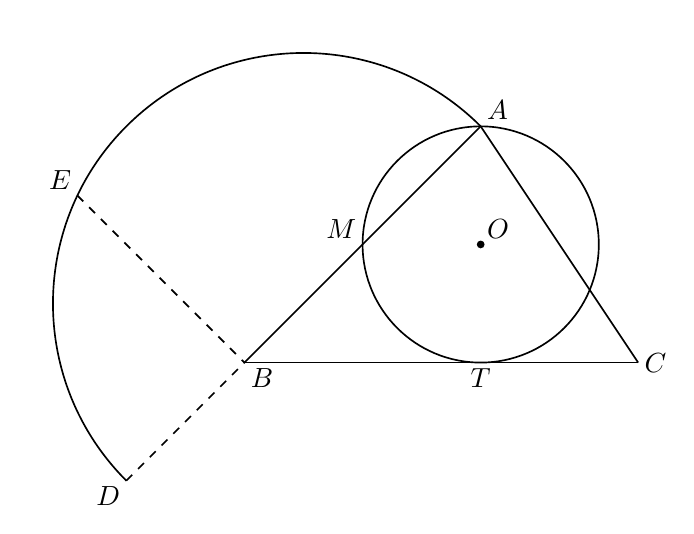
\begin{tikzpicture}[x=1cm,y=1cm,line width=.6pt,font=\normalsize]
\coordinate (B) at (0,0);
\coordinate (A) at (3.0,3.0);
\coordinate (C) at (5.0,0.0);
\coordinate (M) at (1.5,1.5);
\coordinate (T) at (3.0,0.0);
\coordinate (O) at (3.0,1.5);
\coordinate (D) at (-1.5,-1.5);
\coordinate (E) at (-2.1213,2.1213);
\coordinate (Q) at (0.75,0.75);
\draw (O) circle[radius=1.5cm];
\draw (A) arc[start angle=45,end angle=225,radius=3.182cm];
\draw (A)--(B);
\draw (B)--(C);
\draw (A)--(C);
\draw[dashed] (E)--(B);
\draw[dashed] (D)--(B);
\node[above right=2pt,inner sep=0pt] at (A) {$A$};
\node[below right=2pt,inner sep=0pt] at (B) {$B$};
\node[right=2pt,inner sep=0pt] at (C) {$C$};
\node[above left=2pt,inner sep=0pt] at (M) {$M$};
\node[below=2pt,inner sep=0pt] at (T) {$T$};
\node[above right=2pt,inner sep=0pt] at (O) {$O$};
\node[above left=2pt,inner sep=0pt] at (E) {$E$};
\node[below left=2pt,inner sep=0pt] at (D) {$D$};

% Explicit named circle-center points, painted after all region fills.
\fill (O) circle[radius=1.4pt];
\end{tikzpicture}
